\begin{enumerate}
	\item FBA est un triangle équilatéral, donc ses trois angles mesurent 60\textdegree{}.

	ABCD est un carré donc ses quatre angles mesurent 90\textdegree{}.

	Les points F, A et E sont alignés, donc $\widehat{\mathrm{FAE}}=180$\textdegree.

	Ainsi\quad $\widehat{\mathrm{EAD}}=180-90-60=30$\textdegree.

	\item Comme il faut 10 pas pour faire un centimètre dans la réalité, il faut 40 pas pour 4 centimètres :
	\begin{itemize}
		\item \textbf{J} représente la longueur en pas du côté du triangle donc \quad $\textbf{J}=40$;

		\item \textbf{M} représente la longueur en pas du côté du carré donc \quad \textbf{M}=40.
	\end{itemize}

	Pour les rotations, il faut comprendre comment les angles se tracent. Imaginons que notre lutin Scratch est \og orienté à 90\textdegree\fg{}, il regarde donc vers la droite.

	Puis, il avance de 40 pas, et il regarde toujours vers la droite.

	On le fait tourner alors pour qu'il regarde dans la direction du prochain segment.

	\begin{center}
	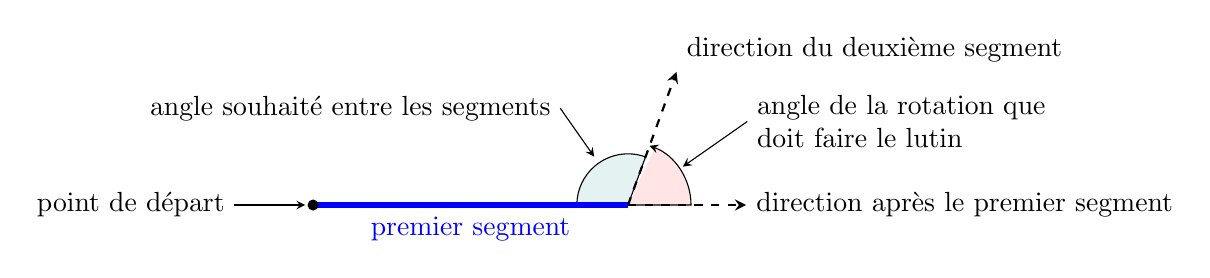
\begin{tikzpicture}[>=stealth]
		\draw[fill=teal!10] (0,0)--(70:0.65) arc (70:180:0.65)--cycle ;
		\draw[<-] (125:0.75)--(125:1.5) node[left]{angle souhaité entre les segments} ;
		\draw[fill=red!10,->] (0,0)--(0:0.8) arc (0:70:0.8) ;
		\draw[<-] (35:0.85)--(35:1.85) node[right,text width=4cm]{angle de la rotation que doit faire le lutin} ;
		\draw[line width=2pt,blue] (-4,0) -- (0,0)node[below,pos=0.5]{premier segment};% -- (70:3)node[right,pos=0.85]{deuxième segment} ;
		\fill (-4,0) circle (2pt);
		\draw[<-] (-4.1,0)--(-5,0)node[left]{point de départ} ;
		\draw[line width=0.8pt,dashed, ->] (0,0) -- (1.5,0) node[right]{direction après le premier segment};
		\draw[line width=0.8pt,dashed, ->] (0,0) -- (70:1.8) node[above right]{direction du deuxième segment};

	\end{tikzpicture}
	\end{center}
	L'angle souhaité entre les segments et l'angle de rotation du lutin Scratch sont donc supplémentaires : leur somme vaut 180\textdegree.

	\begin{itemize}
		\item \textbf{K} représente l'angle de rotation de Scratch, pour un angle souhaité de 60\textdegree entre les segments, donc \quad $\textbf{K}=180 -60 =120$;

		\item \textbf{N} représente l'angle de rotation de Scratch, pour un angle souhaité de 90\textdegree entre les segments, donc  \quad $\textbf{N}=180-90=90$.
	\end{itemize}

	\item Quand le lutin effectue le bloc Triangle, il fait trois rotations de 120\textdegree, et donc il tourne en tout de 360\textdegree : il termine la figure en étant revenu à son point de départ (pour fermer le triangle), en ayant la même orientation qu'au début du bloc.

	De même pour le bloc Carré, car il fait quatre rotations de 90\textdegree : là encore, il est revenu à son point de départ (pour fermer le carré) et il a la même orientation qu'au début du bloc.

	L'instruction \begin{scratch}\blockmove{avancer de \ovalnum{50}pas}\end{scratch} après un bloc Triangle ou Carré nous indique qu'on avance de plus de la longueur d'un côté, qui est de 40 pas, il y aura donc une distance de 10 pas entre le point le plus à droite du premier bloc, et le point de départ du bloc suivant. Cela exclut les figures 1, 2 et 4 (dans la figure 4, on a un espace entre les carrés et les triangles qui suivent, mais pas entre les triangles et les carrés qui les suivent) 	.

	Par ailleurs, l'instruction \begin{scratch}\blockmove{tourner \turnleft{} de \ovalnum{30} degrés}\end{scratch} après chaque bloc Triangle ou Carré crée une figure \og circulaire \fg{} (il y aura en tout 6 rotations de 30 degrés, donc à nouveau 360 degrés en tout); cela confirme la \textbf{figure 3}.
\end{enumerate}
